\documentclass[12pt,a4paper]{article}
\usepackage[utf8]{inputenc}
\usepackage{amsmath}
\usepackage{geometry}
\usepackage{listings}
\usepackage{booktabs}
\usepackage{float}
\usepackage{graphicx}

\geometry{margin=2.5cm}

\lstset{
    basicstyle=\ttfamily\small,
    numbers=left,
    breaklines=true,
    frame=single,
    language=Python,
    tabsize=4
}

\title{\textbf{Report 5: Neural Network with Backpropagation} \\ \large Deep Learning Project 5}
\author{Duong Tan Binh - 2540007}
\date{\today}

\begin{document}

\maketitle
\tableofcontents
\newpage

\section{Introduction}

Labwork~4 showed how a feedforward neural network propagates activations layer by layer,
but the weights were either set by hand or left at random.
\textbf{Backpropagation} is the algorithm that \emph{learns} those weights automatically
by computing how the loss function changes with respect to every parameter in the network
and then applying gradient descent.

This report extends the pure-Python object-oriented implementation from labwork~4
(\texttt{Neuron}, \texttt{Layer}, \texttt{NeuralNetwork}) with a general \texttt{train}
method that performs:
\begin{enumerate}
    \item a \textbf{forward pass} to obtain predictions,
    \item a \textbf{backward pass} to compute gradients via the chain rule, and
    \item a \textbf{weight update} using batch gradient descent.
\end{enumerate}

Two experiments validate the implementation:
\begin{itemize}
    \item \textbf{XOR} --- a non-linearly separable binary classification problem,
          using binary cross-entropy (BCE) loss and a sigmoid output neuron.
    \item \textbf{House price} --- a small regression dataset,
          using mean-squared-error (MSE) loss and a linear output neuron.
\end{itemize}

No external libraries (NumPy, PyTorch, scikit-learn, \ldots) are used.
All arithmetic is performed with Python built-in types and the \texttt{math} module.

\section{Algorithm Description}

\subsection{Forward Pass}

Identical to labwork~4.
Starting from the raw input $\mathbf{a}^{(0)} = \mathbf{x}$, each computational layer
$\ell = 1, \ldots, L$ computes:

\begin{equation}
    z_k^{(\ell)} = \sum_{j=1}^{n^{(\ell-1)}} a_j^{(\ell-1)}\, w_{kj}^{(\ell)} + b_k^{(\ell)},
    \qquad
    a_k^{(\ell)} = f\!\left(z_k^{(\ell)}\right)
    \label{eq:forward}
\end{equation}

where the activation function $f$ is the sigmoid for hidden neurons:
\begin{equation}
    \sigma(z) = \frac{1}{1 + e^{-z}}
    \label{eq:sigmoid}
\end{equation}
and either $\sigma$ (classification) or the identity $f(z)=z$ (regression) for the output.

\subsection{Loss Functions}

\subsubsection{Binary Cross-Entropy (classification)}

For a dataset of $N$ samples with binary targets $y_i \in \{0,1\}$:
\begin{equation}
    J_{\mathrm{BCE}} = -\frac{1}{N} \sum_{i=1}^{N}
        \bigl[y_i \log \hat{y}_i + (1 - y_i) \log (1 - \hat{y}_i)\bigr]
    \label{eq:bce}
\end{equation}

\subsubsection{Mean Squared Error (regression)}

For continuous targets $y_i \in \mathbb{R}$:
\begin{equation}
    J_{\mathrm{MSE}} = \frac{1}{N} \sum_{i=1}^{N} \frac{1}{2}(\hat{y}_i - y_i)^2
    \label{eq:mse}
\end{equation}

\subsection{Backward Pass: Computing Gradients}

The key insight of backpropagation is that the gradient of the loss with respect to
a pre-activation $z_k^{(\ell)}$ --- called the \emph{delta} --- can be computed
recursively from the output layer backwards:

\paragraph{Output layer delta.}
For BCE loss with sigmoid output, the chain rule simplifies elegantly:
\begin{equation}
    \delta_k^{(L)} = \hat{y}_k - y_k
    \label{eq:delta_out_bce}
\end{equation}

For MSE loss with linear output:
\begin{equation}
    \delta_k^{(L)} = \hat{y}_k - y_k
    \label{eq:delta_out_mse}
\end{equation}

Both formulas have the same form; the difference lies in whether $\hat{y}$ was computed
via sigmoid or the identity.

\paragraph{Hidden-layer delta.}
For any layer $\ell < L$, the delta propagates backwards through the weight matrix of
layer $\ell{+}1$ and multiplies by the local sigmoid derivative:
\begin{equation}
    \delta_k^{(\ell)}
    = \left(\sum_{j=1}^{n^{(\ell+1)}} w_{jk}^{(\ell+1)}\, \delta_j^{(\ell+1)}\right)
      \cdot a_k^{(\ell)} \cdot \bigl(1 - a_k^{(\ell)}\bigr)
    \label{eq:delta_hidden}
\end{equation}

The term $a(1-a)$ is the derivative of the sigmoid evaluated at the stored activation ---
no recomputation of $z$ is necessary.

\subsection{Weight Update Rule}

After accumulating deltas over all $N$ samples, the weights are updated with
batch gradient descent:
\begin{equation}
    w_{kj}^{(\ell)} \;\leftarrow\; w_{kj}^{(\ell)}
        - \eta \cdot \frac{1}{N} \sum_{i=1}^{N} a_j^{(\ell-1,i)} \cdot \delta_k^{(\ell,i)}
    \label{eq:update_w}
\end{equation}
\begin{equation}
    b_k^{(\ell)} \;\leftarrow\; b_k^{(\ell)}
        - \eta \cdot \frac{1}{N} \sum_{i=1}^{N} \delta_k^{(\ell,i)}
    \label{eq:update_b}
\end{equation}

where $\eta$ is the learning rate.

\section{Implementation}

\subsection{Neuron class (extended)}

The \texttt{activation} attribute is added to support both sigmoid and linear outputs:

\begin{lstlisting}[caption={Neuron class with configurable activation}]
class Neuron:
    def __init__(self, n_inputs, activation='sigmoid'):
        self.n_inputs   = n_inputs
        self.weights    = [0.0] * n_inputs
        self.bias       = 0.0
        self.z          = 0.0     # pre-activation (cached for backprop)
        self.output     = 0.0     # post-activation
        self.activation = activation   # 'sigmoid' or 'linear'

    @staticmethod
    def sigmoid(z):
        if z >= 0:
            return 1.0 / (1.0 + math.exp(-z))
        e = math.exp(z)
        return e / (1.0 + e)

    def forward(self, inputs):
        self.z = (sum(self.weights[j] * inputs[j]
                      for j in range(self.n_inputs)) + self.bias)
        if self.activation == 'sigmoid':
            self.output = self.sigmoid(self.z)
        else:
            self.output = self.z   # linear output
        return self.output
\end{lstlisting}

\subsection{Backpropagation training loop}

\begin{lstlisting}[caption={train() method – backpropagation core}]
def train(self, X, Y, lr=0.1, epochs=1000, mode='bce'):
    loss_history = []
    N, eps = len(X), 1e-15
    for epoch in range(epochs):
        grad_W = [[[0.0]*len(n.weights) for n in l.neurons]
                  for l in self.layers]
        grad_b = [[0.0]*l.n_neurons for l in self.layers]
        total_loss = 0.0
        for i in range(N):
            # Forward
            activations = [list(X[i])]
            for layer in self.layers:
                activations.append(layer.forward(activations[-1]))
            y_hat = activations[-1][0]
            # Loss
            if mode == 'bce':
                yc = max(eps, min(1-eps, y_hat))
                total_loss += -(Y[i]*math.log(yc)
                                + (1-Y[i])*math.log(1-yc))
            else:
                total_loss += 0.5*(y_hat - Y[i])**2
            # Output delta
            deltas = [None]*len(self.layers)
            deltas[-1] = [y_hat - Y[i]]   # same form for BCE+sigmoid / MSE+linear
            # Hidden deltas (right to left)
            for l in range(len(self.layers)-2, -1, -1):
                nxt = self.layers[l+1]
                deltas[l] = [
                    sum(nxt.neurons[j].weights[k]*deltas[l+1][j]
                        for j in range(nxt.n_neurons))
                    * activations[l+1][k] * (1 - activations[l+1][k])
                    for k in range(self.layers[l].n_neurons)
                ]
            # Accumulate gradients
            for l, layer in enumerate(self.layers):
                for k, neuron in enumerate(layer.neurons):
                    for j in range(len(neuron.weights)):
                        grad_W[l][k][j] += activations[l][j]*deltas[l][k]
                    grad_b[l][k] += deltas[l][k]
        # Update
        for l, layer in enumerate(self.layers):
            for k, neuron in enumerate(layer.neurons):
                for j in range(len(neuron.weights)):
                    neuron.weights[j] -= lr*grad_W[l][k][j]/N
                neuron.bias -= lr*grad_b[l][k]/N
        loss_history.append(total_loss/N)
    return loss_history
\end{lstlisting}

Key implementation points:
\begin{itemize}
    \item \textbf{Activation caching}: after each forward call, \texttt{neuron.output}
          holds $a_k^{(\ell)}$, which is reused directly in the sigmoid derivative
          $a(1-a)$ --- no extra computation needed.
    \item \textbf{Same delta formula}: for BCE + sigmoid output and MSE + linear output,
          the per-sample output delta reduces to $\hat{y} - y$.
    \item \textbf{He initialisation}: weights drawn from
          $\mathcal{N}(0,\; \sqrt{2/n_{\mathrm{in}}})$,
          biases set to zero.
    \item \textbf{Pure Python}: only \texttt{math}, \texttt{random},
          and \texttt{matplotlib} are imported.
\end{itemize}

\section{Experiment 1: XOR Dataset}

\subsection{Dataset}

XOR is the canonical non-linearly separable binary function.
No single sigmoid neuron can draw a straight decision boundary separating the two classes.

\begin{table}[H]
\centering
\caption{XOR truth table}
\begin{tabular}{ccc}
\toprule
$x_1$ & $x_2$ & $y$ \\
\midrule
0 & 0 & 0 \\
0 & 1 & 1 \\
1 & 0 & 1 \\
1 & 1 & 0 \\
\bottomrule
\end{tabular}
\end{table}

\subsection{Architecture and Initialisation}

Architecture: $[2 \to 4 \to 1]$ --- two input features, one hidden layer with four sigmoid
neurons, one sigmoid output neuron.
Weights initialised with He initialisation (seed = 42), biases = 0.

\begin{table}[H]
\centering
\caption{XOR network configuration}
\begin{tabular}{llll}
\toprule
Layer & Neurons & Activation & Parameters \\
\midrule
Input  & 2 & ---      & --- \\
Hidden & 4 & sigmoid  & $4 \times (2 + 1) = 12$ \\
Output & 1 & sigmoid  & $1 \times (4 + 1) = 5$ \\
\midrule
Total  &   &          & \textbf{17} \\
\bottomrule
\end{tabular}
\end{table}

\subsection{Intermediate Steps}

To verify convergence, training with learning rate $\eta = 1.0$ is traced at intervals
of 1000 epochs:

\begin{table}[H]
\centering
\caption{XOR training progress ($\eta = 1.0$, 5000 epochs)}
\begin{tabular}{rr}
\toprule
Epoch & BCE Loss \\
\midrule
1000 & 0.019253 \\
2000 & 0.005294 \\
3000 & 0.002981 \\
4000 & 0.002059 \\
5000 & 0.001568 \\
\bottomrule
\end{tabular}
\end{table}

The loss decreases monotonically, confirming that gradient descent is working correctly.

\subsection{Effect of Different Learning Rates}

Four learning rates are compared over 5000 epochs with identical initialisation (seed = 42):

\begin{table}[H]
\centering
\caption{XOR – final BCE loss and accuracy for different learning rates}
\begin{tabular}{rrrl}
\toprule
$\eta$ & Final BCE Loss & Accuracy & Notes \\
\midrule
0.1 & 0.277813 & 4/4 = 100\% & Converges slowly \\
0.5 & 0.003826 & 4/4 = 100\% & Good convergence \\
1.0 & 0.001568 & 4/4 = 100\% & Faster convergence \\
2.0 & \textbf{0.000706} & \textbf{4/4 = 100\%} & \textbf{Best} \\
\bottomrule
\end{tabular}
\end{table}

All four learning rates eventually achieve 100\% accuracy; the difference is the speed and
tightness of convergence.
A higher $\eta$ converges faster here because the XOR problem is well-conditioned and the
network architecture has enough capacity.

\begin{figure}[H]
\centering
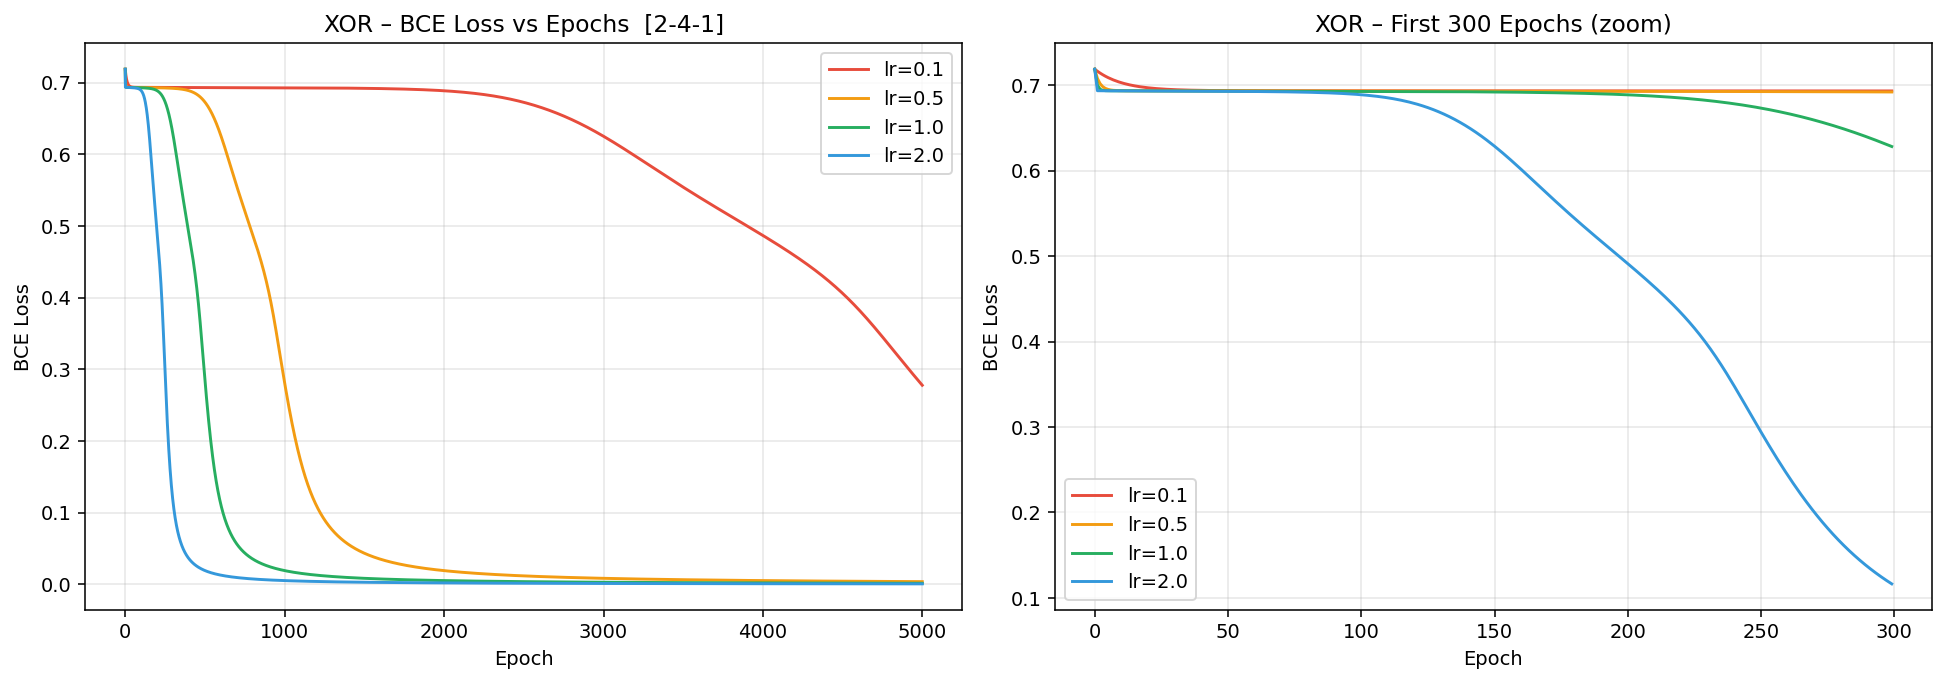
\includegraphics[width=\textwidth]{backprop_xor_loss.png}
\caption{Left: BCE loss over 5000 epochs for four learning rates.
Right: zoom into the first 300 epochs showing that $\eta=0.1$ (red) starts converging
much later than the other rates.}
\end{figure}

\subsection{Final Results}

Best model: $\eta = 2.0$ after 5000 epochs.

\begin{table}[H]
\centering
\caption{XOR predictions after backpropagation training ($\eta=2.0$)}
\begin{tabular}{ccrrrc}
\toprule
$x_1$ & $x_2$ & Expected & Output $\hat{y}$ & Prediction & Correct? \\
\midrule
0 & 0 & 0 & 0.0008 & 0 & \textbf{Yes} \\
0 & 1 & 1 & 0.9993 & 1 & \textbf{Yes} \\
1 & 0 & 1 & 0.9993 & 1 & \textbf{Yes} \\
1 & 1 & 0 & 0.0006 & 0 & \textbf{Yes} \\
\bottomrule
\end{tabular}
\end{table}

Accuracy: $4/4 = 100\%$.
The outputs are now extremely close to the ideal $\{0, 1\}$ values --- very different from
the hand-set weights in labwork~4 which only achieved $50\%$ accuracy.

\begin{figure}[H]
\centering
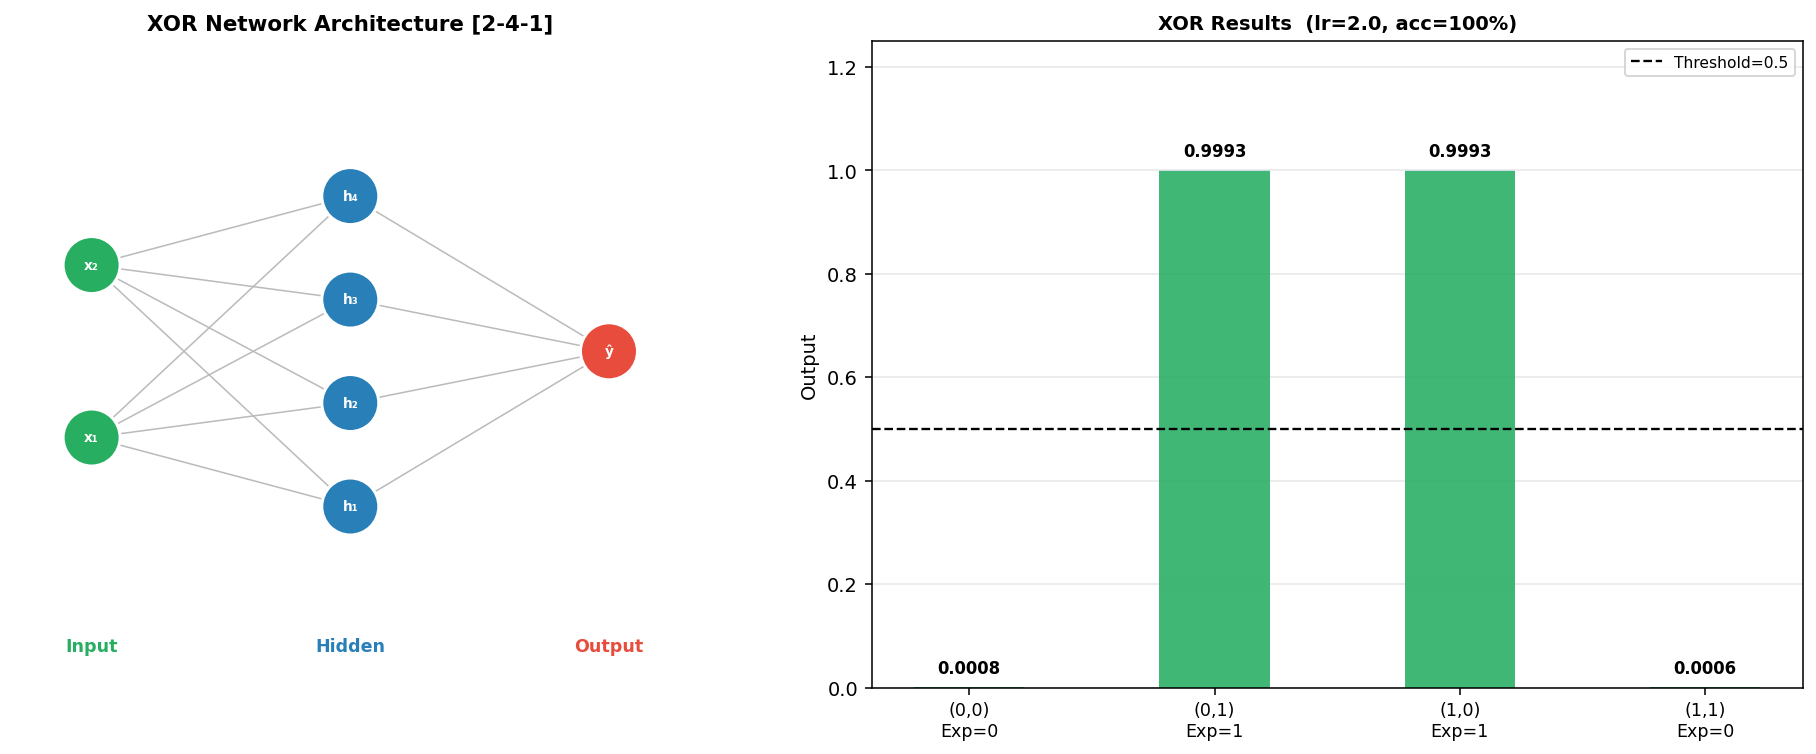
\includegraphics[width=\textwidth]{backprop_xor_results.png}
\caption{Left: XOR network architecture [2-4-1].
Right: network outputs (green bars = correct) vs.\ expected values (transparent blue).
All four inputs are classified correctly with outputs very close to 0 or 1.}
\end{figure}

\begin{figure}[H]
\centering
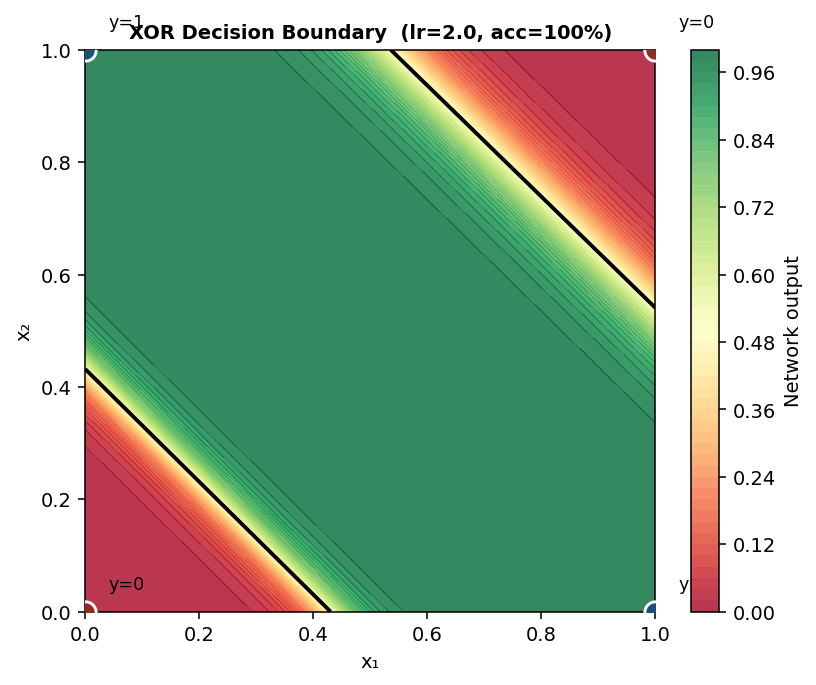
\includegraphics[width=0.7\textwidth]{backprop_xor_decision.png}
\caption{Decision boundary learned by the network.
The background colour shows the network output (green $\approx 1$, red $\approx 0$).
The solid black contour marks the 0.5 threshold.
Blue dots = class 1, red dots = class 0 --- all four XOR points are on the correct
side of the boundary.}
\end{figure}

\section{Experiment 2: House Price Dataset}

\subsection{Dataset}

A small dataset of five house size–price pairs, loaded from \texttt{house\_price.csv}
following the project's standard file-reading pattern.

\begin{table}[H]
\centering
\caption{House price dataset}
\begin{tabular}{cc}
\toprule
Size (m\textsuperscript{2}) & Price (unit) \\
\midrule
10 & 55 \\
20 & 80 \\
40 & 100 \\
60 & 120 \\
80 & 150 \\
\bottomrule
\end{tabular}
\end{table}

Both input and output are normalised to $[0, 1]$:

\[
    x_{\mathrm{norm}} = \frac{x - x_{\min}}{x_{\max} - x_{\min}}, \quad
    y_{\mathrm{norm}} = \frac{y - y_{\min}}{y_{\max} - y_{\min}}
\]

with $x_{\min} = 10,\; x_{\max} = 80,\; y_{\min} = 55,\; y_{\max} = 150$.

\subsection{Architecture and Configuration}

Architecture: $[1 \to 4 \to 1]$ --- one input feature, four hidden sigmoid neurons,
one \textbf{linear} output neuron (appropriate for regression).
Loss function: MSE (Equation~\eqref{eq:mse}).
Weights initialised with He initialisation (seed = 0), biases = 0.

\subsection{Intermediate Steps}

Training progress for $\eta = 0.1$:

\begin{table}[H]
\centering
\caption{House price training progress ($\eta=0.1$, 3000 epochs, normalised MSE)}
\begin{tabular}{rr}
\toprule
Epoch & MSE Loss \\
\midrule
600  & 0.001667 \\
1200 & 0.001368 \\
1800 & 0.001351 \\
2400 & 0.001335 \\
3000 & 0.001321 \\
\bottomrule
\end{tabular}
\end{table}

\subsection{Effect of Different Learning Rates}

\begin{table}[H]
\centering
\caption{House price – final MSE (normalised) for different learning rates}
\begin{tabular}{rrl}
\toprule
$\eta$ & Final MSE & Notes \\
\midrule
0.01 & 0.008800 & Too slow, not yet converged \\
0.05 & 0.001359 & Good \\
0.10 & 0.001321 & Better \\
0.50 & \textbf{0.001195} & \textbf{Best} \\
\bottomrule
\end{tabular}
\end{table}

\begin{figure}[H]
\centering
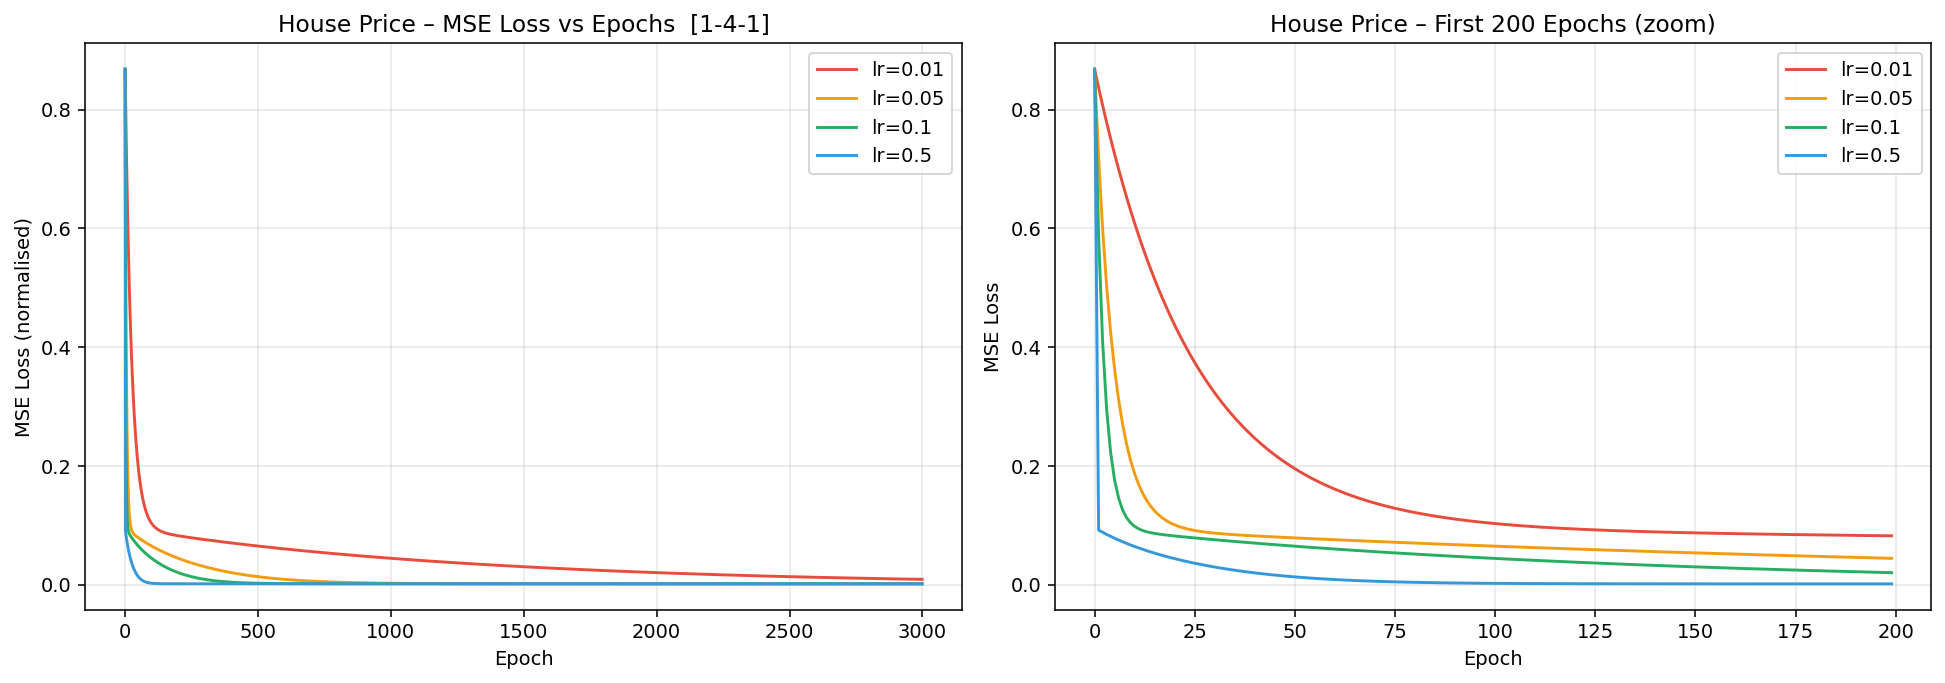
\includegraphics[width=\textwidth]{backprop_house_loss.png}
\caption{Left: normalised MSE loss over 3000 epochs for four learning rates.
Right: zoom into the first 200 epochs showing the initial rapid descent for larger $\eta$.
$\eta = 0.01$ (red) has not converged after 3000 epochs, while $\eta = 0.5$ (blue)
reaches the lowest loss.}
\end{figure}

\subsection{Final Results}

Best model: $\eta = 0.5$ after 3000 epochs.
Predictions are denormalised back to original price units.

\begin{table}[H]
\centering
\caption{House price predictions after backpropagation training ($\eta=0.5$)}
\begin{tabular}{crrr}
\toprule
Size (m\textsuperscript{2}) & True Price & Predicted Price & Absolute Error \\
\midrule
10 & 55.0 & 59.60 & 4.60 \\
20 & 80.0 & 73.02 & 6.98 \\
40 & 100.0 & 100.09 & 0.09 \\
60 & 120.0 & 125.35 & 5.35 \\
80 & 150.0 & 146.95 & 3.05 \\
\bottomrule
\end{tabular}
\end{table}

The largest absolute error is $\approx 7$ units for the size-20 house.
The prediction at size 40 (the midpoint) is nearly perfect ($\approx 0.09$ error),
which shows that the network learns the underlying trend well despite the small dataset.

\begin{figure}[H]
\centering
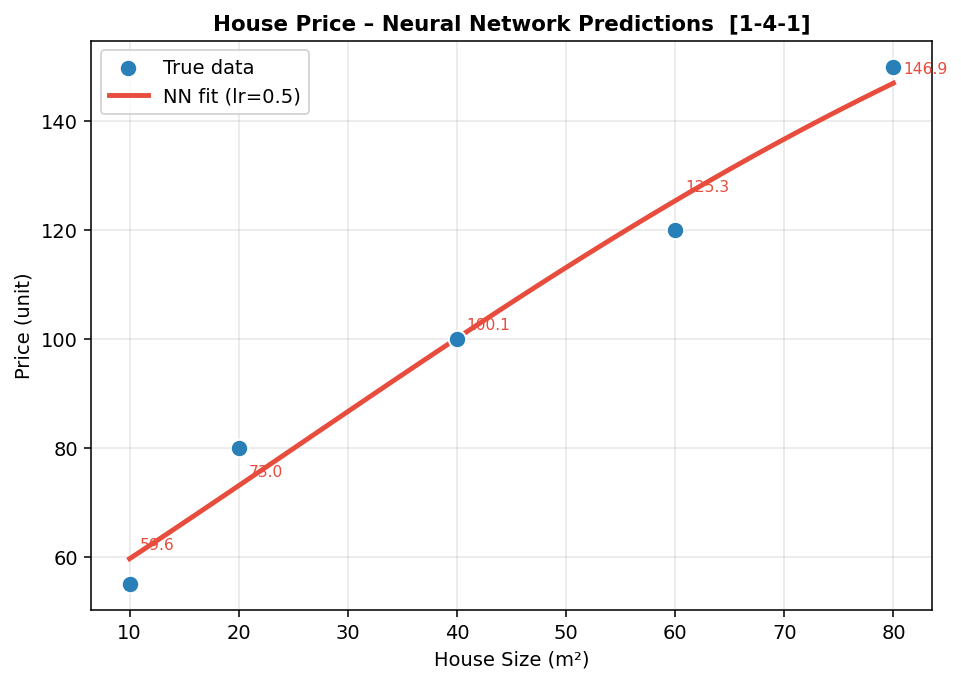
\includegraphics[width=0.75\textwidth]{backprop_house_predictions.png}
\caption{Blue dots: true data points.
Red curve: neural network fit (predictions at 100 uniformly spaced size values).
Red annotations: predicted price at each training point.
The network captures the roughly linear trend in the data.}
\end{figure}

\section{Conclusion}

I extended the feedforward network from labwork~4 with a general backpropagation
training method, implemented entirely in pure Python.
The key outcomes are:

\begin{enumerate}
    \item \textbf{Correct gradient computation.}
          For BCE loss with sigmoid output, the output delta simplifies to
          $\hat{y} - y$; for MSE with linear output it has the same form.
          Hidden-layer deltas propagate backwards via the chain rule using the stored
          activations and the sigmoid derivative $a(1-a)$.

    \item \textbf{XOR solved perfectly.}
          After 5000 epochs of batch gradient descent with $\eta = 2.0$, the $[2\to4\to1]$
          network achieves 100\% accuracy with outputs
          $(0.0008,\; 0.9993,\; 0.9993,\; 0.0006)$ ---
          extremely close to the ideal $\{0,1\}$ targets.
          This is a dramatic improvement over the hand-set weights in labwork~4
          which only reached 50\% accuracy.

    \item \textbf{Regression on house price.}
          The $[1\to4\to1]$ network with a linear output neuron and MSE loss
          fits the size-to-price relationship with a maximum absolute error of $\approx 7$
          price units and near-zero error at the central data point.

    \item \textbf{Learning rate effect.}
          For XOR, a larger $\eta$ converges faster; for the small house-price dataset,
          $\eta = 0.5$ produces the lowest MSE.
          Learning rate $\eta = 0.01$ fails to converge within 3000 epochs, confirming
          that an appropriate learning rate is critical.

    \item \textbf{General implementation.}
          The \texttt{train} method supports any network depth, any combination of
          hidden-layer widths, and two modes (\texttt{bce} / \texttt{mse}), making it
          easy to experiment without changing any code.
\end{enumerate}

\end{document}
